\documentclass{article}

\usepackage{ctex}
\usepackage[left=1.25in,right=1.25in,top=1in,bottom=1in]{geometry}
\usepackage{amsmath}
\usepackage{amssymb}
\usepackage{graphicx}
\usepackage{listings}
\lstset{language=Matlab}   
\lstset{breaklines}              
\lstset{extendedchars=false}
\usepackage[framed,numbered,autolinebreaks,useliterate]{mcode}

\author{张泽宇}
\date{2022年3月13日}
\title{第三周工作总结}

\begin{document}
	\maketitle
	
	{\centering \rule[15pt]{15cm}{0.1em}}
	
	{\noindent\large\textbf{
	这一周的主要进行的工作包括有:
	\begin{itemize}
		\item 对上周仿真模型进行改进,添加了故障电阻,去掉了电路中不必要的部分,使电路更为简单。
		\item 补充了正常情况下的数据集,包括正常情况下负载不同时电流波形,不同故障电阻下负载的故障电流。
		\item 对神经网络进行了调整,主要体现在网络超参数的设定,进行了不同的尝试。同时编写了command window接口程序,用训练集和验证集之外生成的图片进行了测试。
		\item 参照资料学习并搭建了一个简单的三相电路,进行了初步学习。
	\end{itemize}}}

	以下为详细叙述
	
	{\centering \rule[-10pt]{15cm}{0.1em}}
	
	\section{仿真模型改进}
	
	\subsection{电路结构调整}
	
	我听取了教授关于故障电阻的建议,在全波整流电路中某一桥臂上添加了一个故障电阻,这个电阻为可变电阻,受到脉冲信号的控制,在第0.06s时由0$\Omega$变为200$\Omega$.
	
	这我有一个疑问,就是关于故障电阻,我的理解是通过调节故障电阻的值,可以模拟线路发生不同情况下产生的多余阻抗,比如输电线绝缘层的破损程度不同,产生的阻抗也就不同,这就可以很好的用故障电阻表示。但是在像我这个模型中的电子电路里,故障电阻最多只能模拟短路和开路的情况,调节它的阻值是否有现实的意义?还是只是为了获得不同情型下的电流波形。
	
	另外,在构造故障电阻模型的过程中,我使用的是可调电阻Variable Resistor加阶跃信号Step两个模块,这样虽然可以在0.06s时模拟出故障发生,但是不同的阻值需要手工设定,想要获得多一些的数据,比如10组20组,或者更多的地方需要修改数值,可能就得费点事情。有没有其他方便的方法或者模块可以在simulink中使用?
	
	\subsection{仿真时间的调整}
	
	我按照教授给出的建议,将仿真时间调整到10ms,在第6ms的时候故障发生。在50赫兹的工频下,这样可以根据故障发生后两个周期的波形改变判断是否发生故障。
	
	\section{补充了正常情况下的数据集}
	
	通过调整负载电阻不同的阻值,得到负载电流随负载大小变化的一系列正常与故障样本。然后再在上周的数据拓展方面进行进一步的处理,得到了近1200张相关的图片。在数据集的制作方面,我总结得出的模式就是“matlab仿真+python数据增强”。
	
	\begin{figure}[htpb]
		\centering
		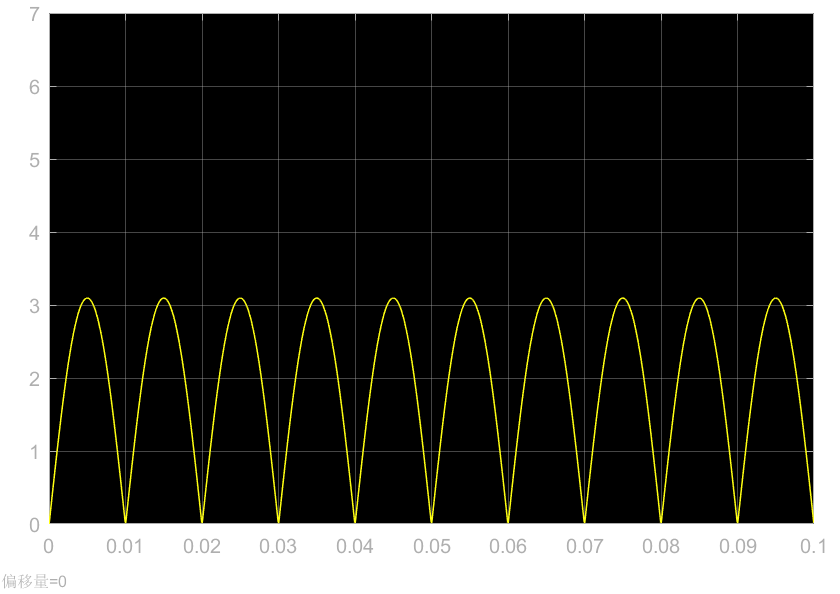
\includegraphics[width=7cm]{figure/normal_100ohms.png}
		\quad
		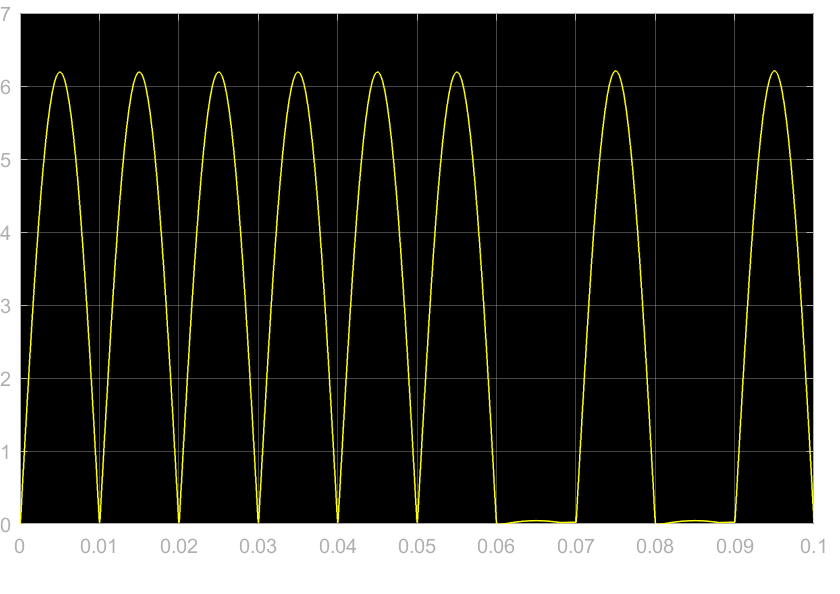
\includegraphics[width=7cm]{figure/D2_short_60ms_50ohms.png}
		\caption{部分正常与故障图像}
	\end{figure}

	但是,在这一方面也存在着和之前类似的问题,负载电阻无法实现自动的阻值调整,依旧需要手工修改设定。当需要调整的量较大时,比较费时费力。
	
	\section{对神经网络进行调整}
	
	\subsection{调参}
	我查阅了一些资料,对神经网络的调参方法与调参技巧进行了一些学习。主要的调参过程和原则如下:
	
	\begin{enumerate}
		\item 恰好拟合时,训练集和测试集的LOSS都已经收敛,且很接近,模型能够很好地拟合训练样本和测试样本,泛化能力强。此时需要以优化网络设计为方向调整参数,使达到同样的效果下,网络结构更小、更轻量。
		
		主要的方法可以有:
		\begin{itemize}
			\item 减少网络层数
			\item 减少不同的层的参数,主要是卷积核的数量
			\item 适当调大batchsize(但这个尝试之后不太行,显示出计算机内存不够的提示)
		\end{itemize}
	
		\item 欠拟合时,从LOSS曲线上看,训练集和测试集从趋势上还没有收敛。可以做的调整是:
		
		\begin{itemize}
			\item 增加数据集,进行数据清洗
			\item 加大训练迭代次数,有可能是网络还没训练完
			\item 进一步衰减调小学习率
			\item 添加更多的层,也有可能是网络容量不够
			\item 去掉正则化约束的部分,L1、L2正则(正则主要是为了防止过拟合)
			\item 加入BN层加快收敛速度
			\item 增加网络的非线性度(ReLu)
		\end{itemize}
	
		\item 过拟合:从LOSS曲线上看,都趋向收敛,但是测试集上的LOSS很高,甚至出现回升现象。说明泛化能力差,有可能训练集和测试集数据分布不一致,更加可能的是模型太复杂。可以调整的有:
		
		\begin{itemize}
			\item 增加样本数量,训练样本太少或者说小样本问题,很容易导致过拟合。
			\item 数据增强
			\item 早停法(Early stopping),从LOSS不在下降的地方拿到模型,作为训练好的模型
			\item 降低网络的复杂度(深度)
			\item L1 regularization,L2 regulariztion
			\item Dropout策略
			\item 适当降低Learning rate
			\item 适当减少epoch的次数
		\end{itemize}
		
		\item 完全不收敛,LOSS一直都很高。
			\begin{itemize}
				\item 先检查数据,输入数据、预处理、数据增强、标签等
				\item 网络设计或者参数使用错误
				\item LOSS设计,优化函数
			\end{itemize}
	\end{enumerate}

	具体到这个模型中来看,经过许多次的调节后,确实达到了一个很好的水平,基本上满足了完全拟合的要求,准确率提升到了95\%以上,甚至有几次迭代过后能够达到100\%。当然,这也和需要解决的问题太过简单有关,正常和故障时的负载电流图像之间差别很大。
	
	\begin{figure}[htpb]
		\centering
		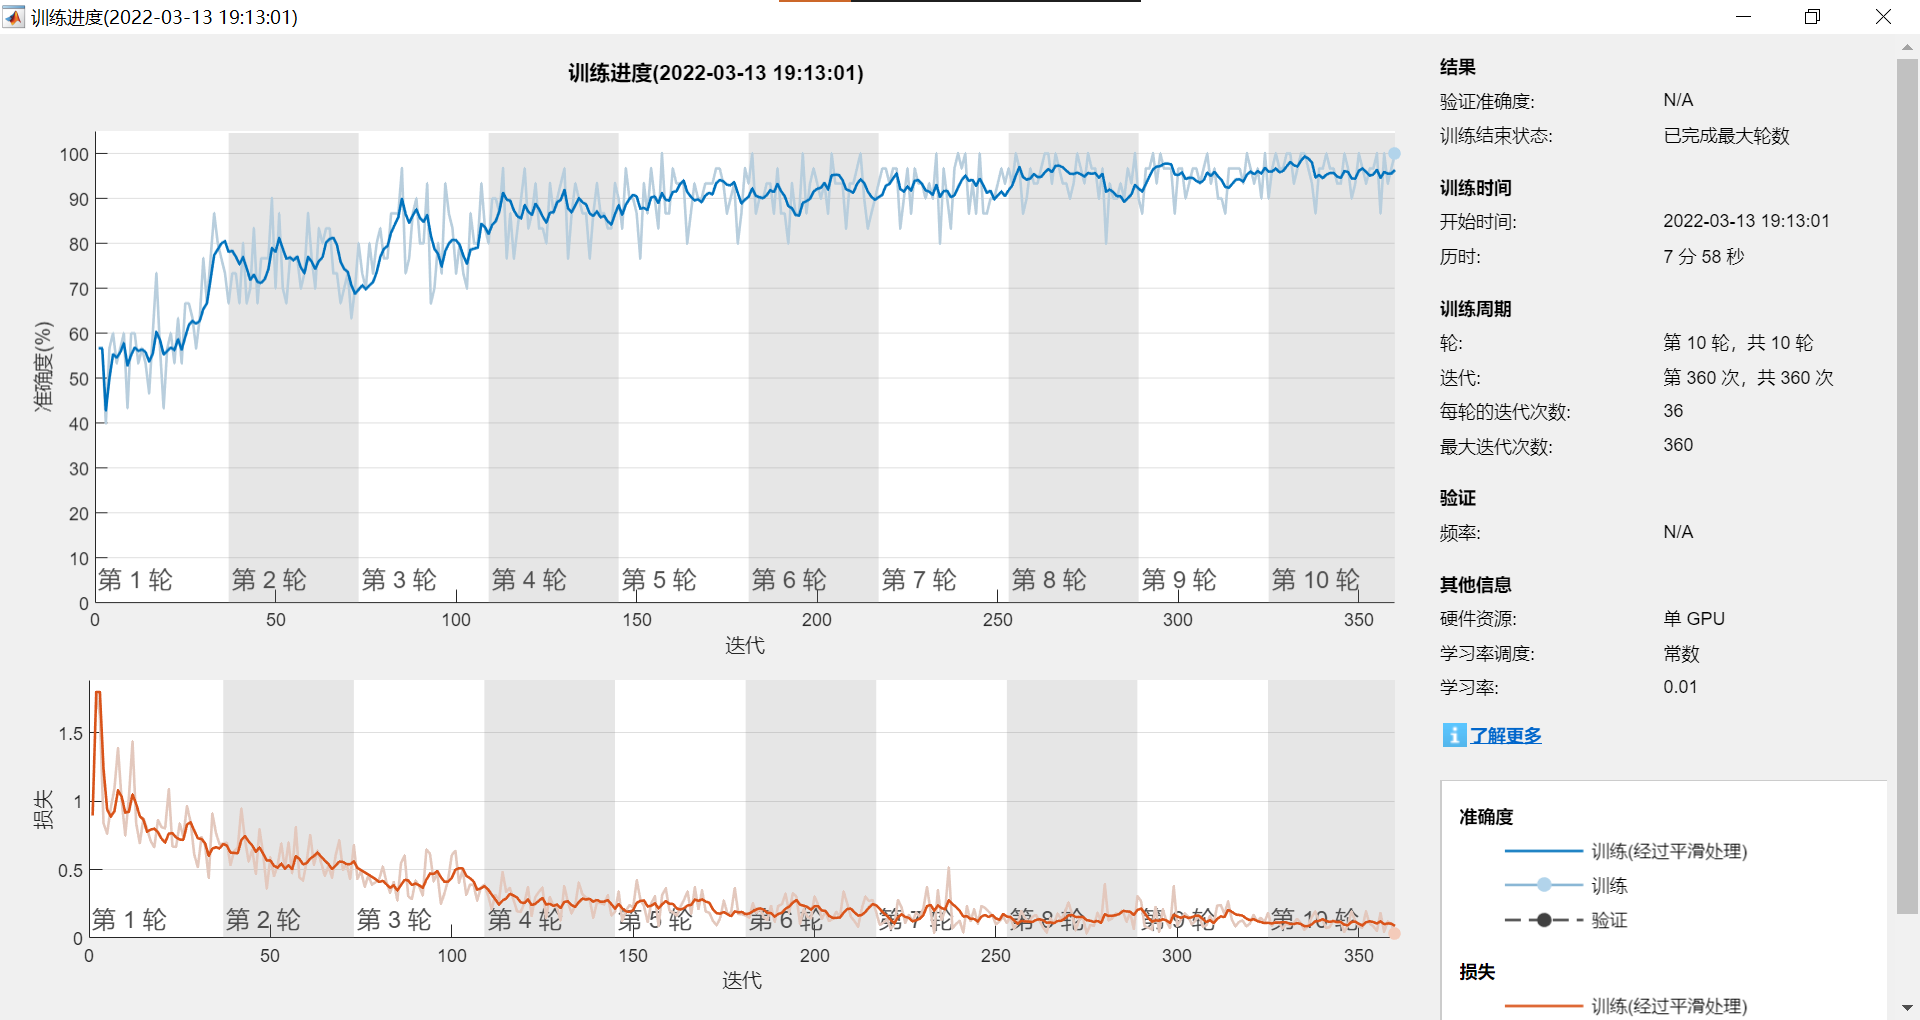
\includegraphics[width=10cm]{figure/2nd.png}
		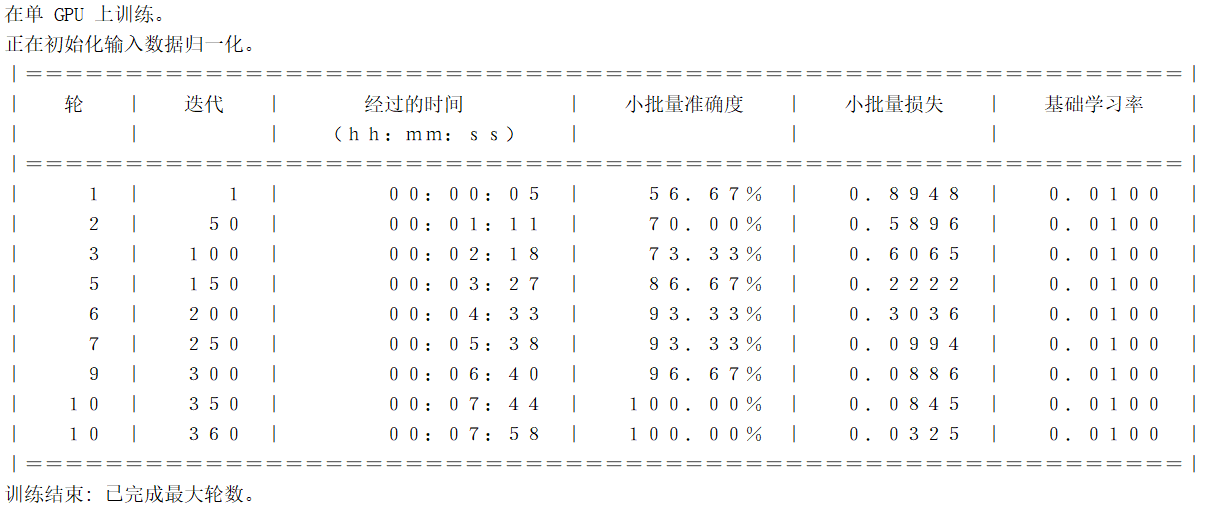
\includegraphics[width=10cm]{figure/2nd_table.png}
		\caption{最终的训练结果}
	\end{figure}
	
	对比来看,当学习率调高一些,到0.02时,训练效果明显下降,出现了欠拟合,无法收敛的现象。
	
	\begin{figure}[htpb]
		\centering
		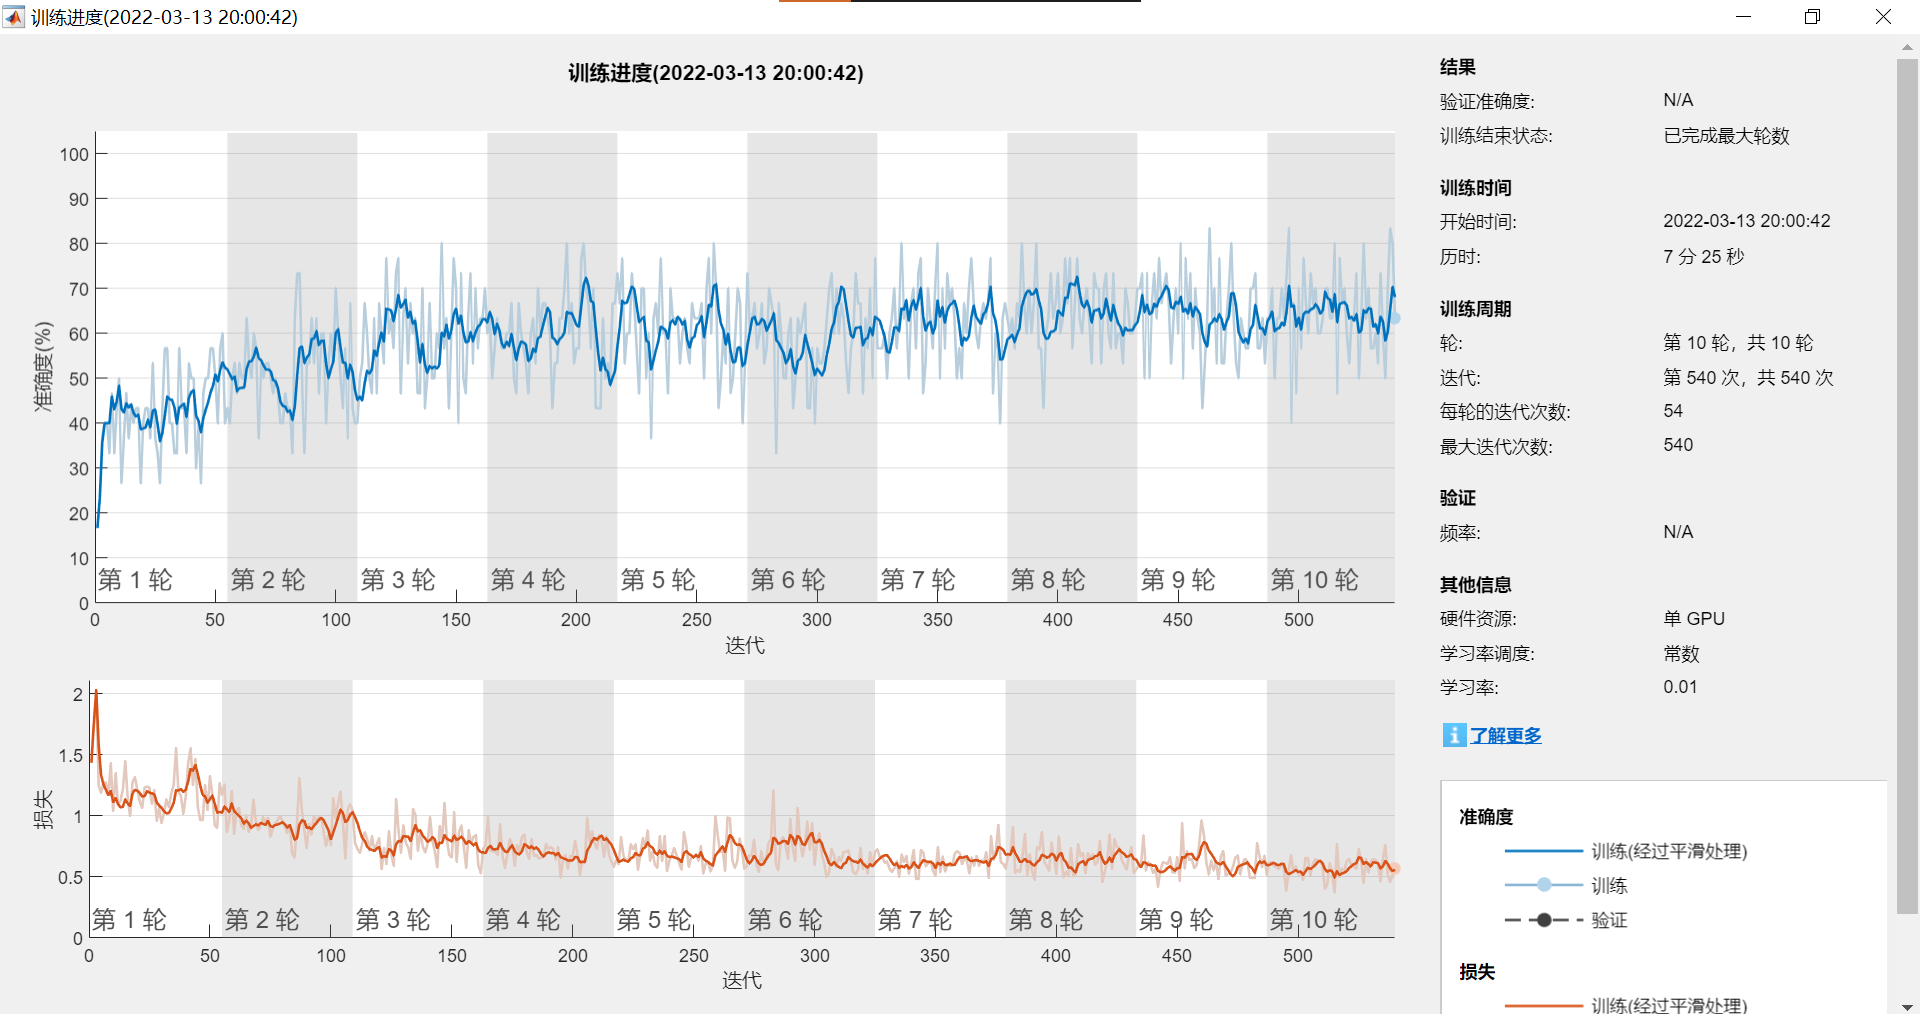
\includegraphics[width=10cm]{figure/4th.png}
		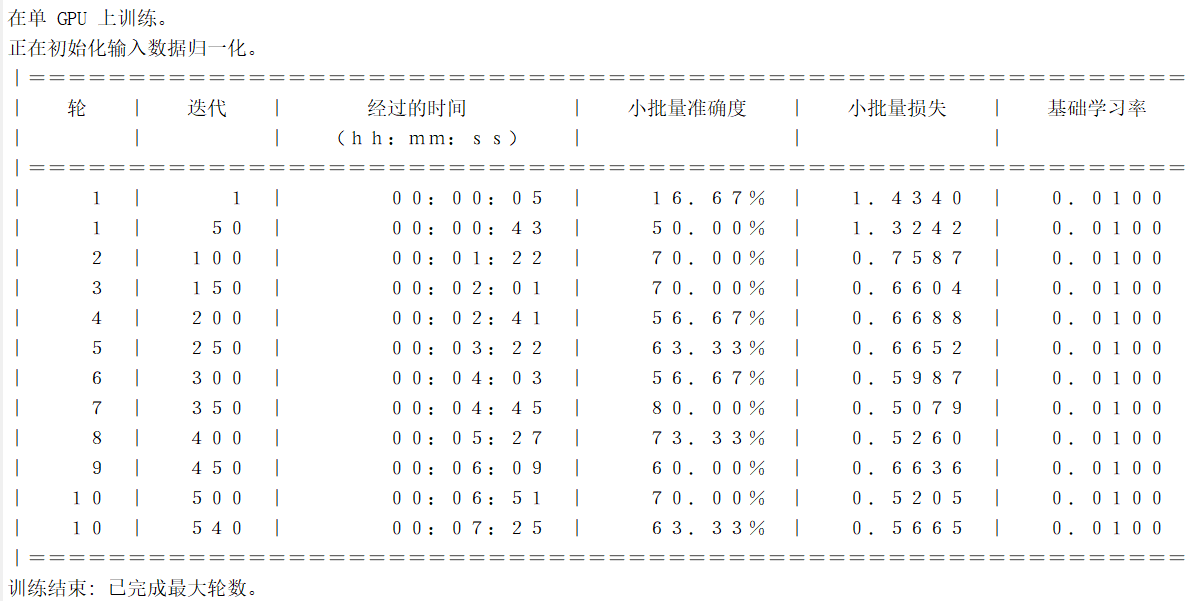
\includegraphics[width=10cm]{figure/4th_table.png}
		\caption{学习率调整到0.02后出现欠拟合}
	\end{figure}
	
	尽管如此,网络仍旧存在有训练时间过长的问题,单次训练需要7至8分钟不等。网络在结构设计方面仍然需要进行改动。
	
	\subsection{command window接口}
	
	把训练之后的网络保存,然后在command window中输入要检测的图片路径,就可以直接判断出这个图片属于怎样的故障。经过实际测试,预测结果较好。
	
	\begin{figure}[htpb]
		\centering
		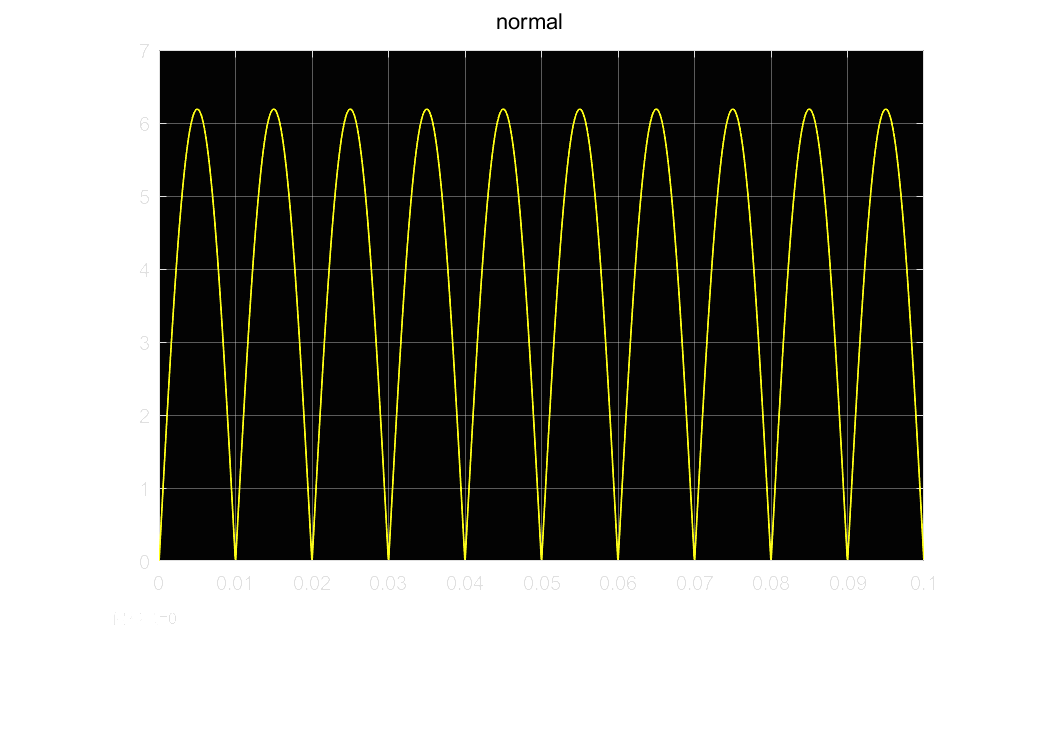
\includegraphics[width=10cm]{figure/training_result.png}
		\caption{预测结果}
	\end{figure}

	程序代码:
	
	\begin{lstlisting}
	clear;
	load fault_detection_try;
	
	file_name = '';
	im = imread(file_name);
	figure();
	im = imresize(im,[594 840]);
	imshow(im);
	prediction = classify(net,im);
	title(char(prediction));
	\end{lstlisting}
	
	\section{简单的三相电路}
	
	我参照文献《MATLAB/Simulink仿真在电力系统短路故障中的应用》\footnote{王瀚,周海峰,刘天熙,黄金满,郑聪.MATLAB/Simulink仿真在电力系统短路故障中的应用[J].应用能源技术,2020(07):1-8.},简单学习搭建了一个无限大功率电力系统仿真模型。
	
	\begin{figure}[htpb]
		\centering
		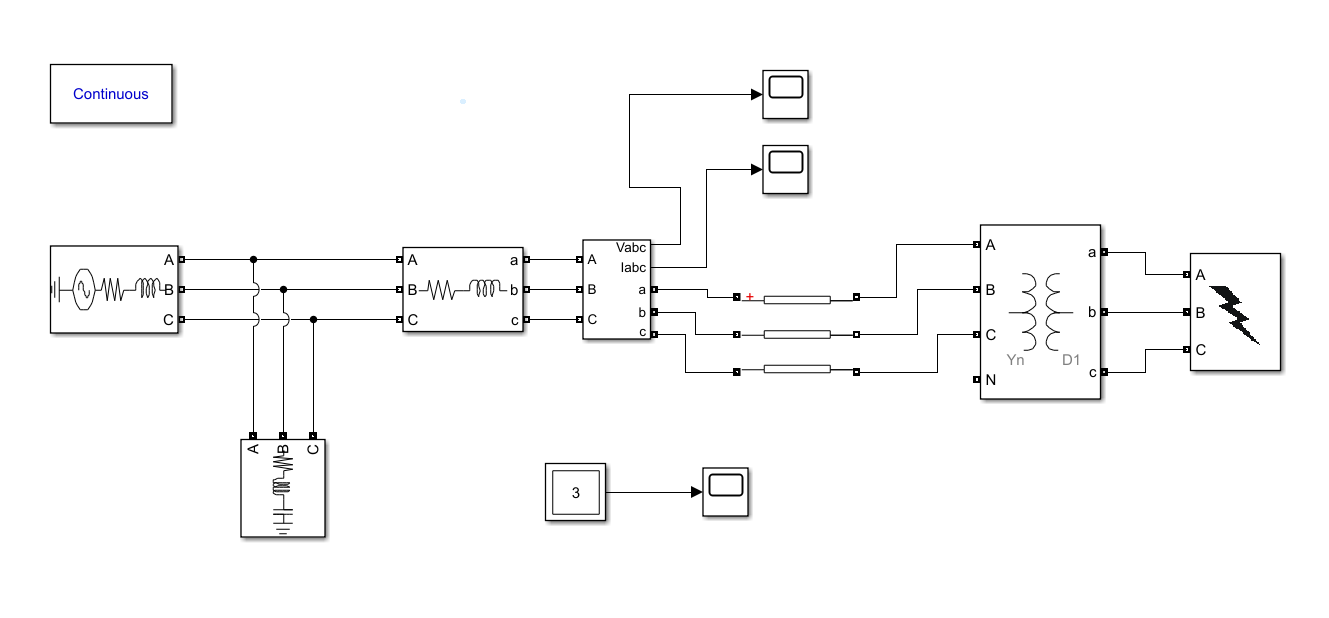
\includegraphics[width=13cm]{figure/three_phase.png}
		\caption{无限大功率电力系统仿真}
	\end{figure}

	并且利用Three-Phase Fault模块设置了相地之间、两相之间的短路故障,基本上复现了文章里出现的仿真情况。
	
	\begin{figure}[htpb]
		\centering
		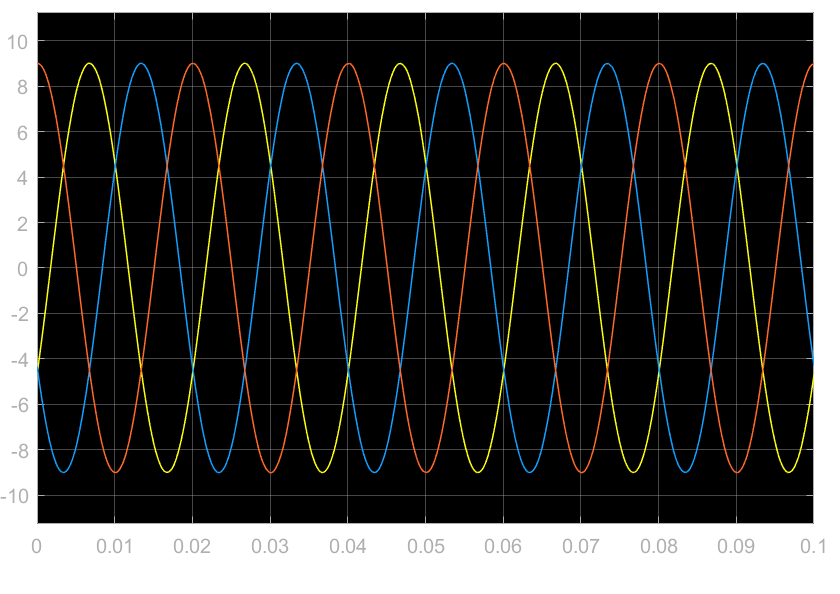
\includegraphics[width=7cm]{figure/normal_three_phase.png}
		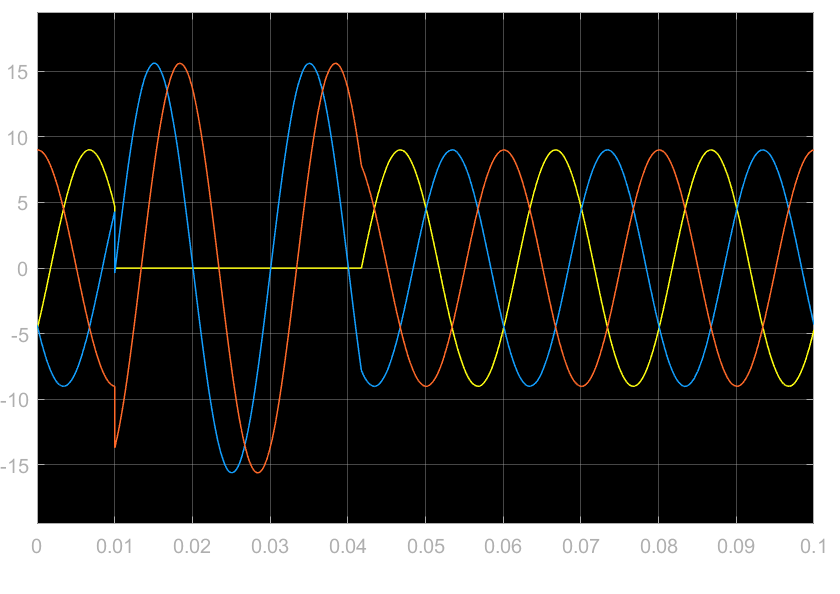
\includegraphics[width=7cm]{figure/A_ground_short_three_phase.png}
		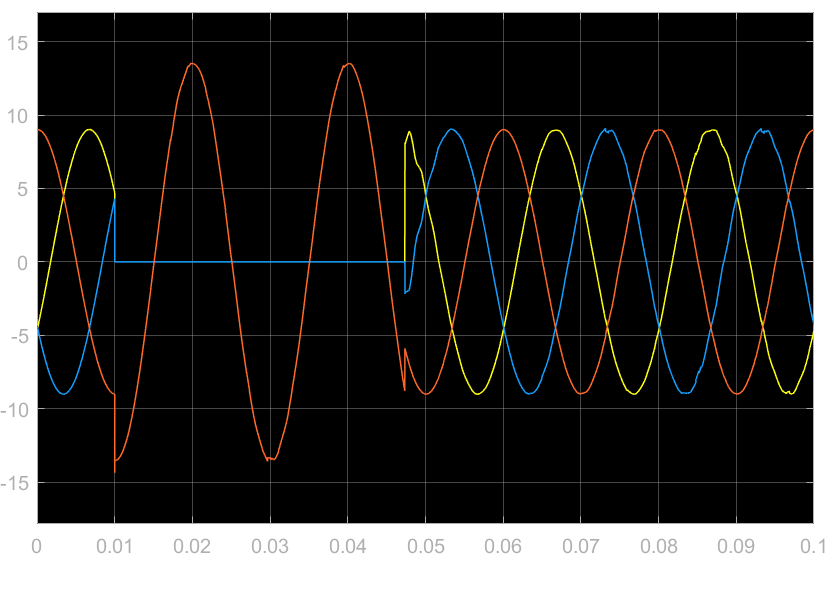
\includegraphics[width=7cm]{figure/A_B_short_three_phase.png}
		\caption{正常情况、A相对地短路、AB相间短路}
	\end{figure}
	但是这一个系统的学习需要下周更为深入的了解。
	
	\section{下周计划}
	
	\begin{enumerate}
		\item 对第二周开始的全波整流电路故障检测神经网络进行最后的整理和完善。
		\item 就无限大功率电力系统原理进行学习。
		\item 寻找参考一些已有的故障检测神经网络程序,进行学习。
	\end{enumerate}
\end{document}